% !Mode\dots ``TeX:UTF-8''
% !TEX root = ../bare_jrnl.tex
\section{The online observability of \BCNs}
\label{sec:online}

In this section we propose the online observability to solve the problem mentioned in {\em Section \ref{sec:pre}}, and we will introduce its related information in detail. 

In the rest of this section, firstly we introduce the inspiration for the online observability. Secondly we define derivation function. Thirdly we present the definition of $k$-step determinability. Finally, we give the formal definition of the online observability of \BCNs\ by derivation function and $k$-step determinability, and compare it with four existing observability.

\subsection{Inspiration}


As we mentioned in {\em Section \ref{sec:pre}}, we can determine the initial states of \BCNs\ by the third existing observability. But in the third observability, a \BCN\ is observable unless there exists an finite input sequence $\mathsf{I}\in(\Delta_M)^k$ that determine its initial state $\mathsf{s}(0)$. 

However, as we can derive the set of possible initial states $\mathsf{S}(0)$ by initial output $\mathsf{o}(0)$ we observe
\[\mathsf{S}(0)=\{\mathsf{s}(0)|\mathsf{s}(0)\in \Delta_N\ ,\ h( \mathsf{s}(0))=\mathsf{o}(0)\}.\]
And if for every $\mathsf{S}^{i}(0)$ (corresponding to the $\mathsf{o}^{i}(0)$) we derived, there is an input sequence $\mathsf{I}^{i}\in(\Delta_M)^k$ for some $k>0$, such that for any distinct states $\mathsf{s}^{x}(0)$, $\mathsf{s}^{y}(0) \in \mathsf{S}^{i}(0)$ implies $(HF)^k_{\mathsf{s}^{x}(0)}(\mathsf{I^i})\neq (HF)^k_{\mathsf{s}^{y}(0)}(\mathsf{I^i})$,
then we can determine the initial state too. 
What is more, in this case, the requirements for a \BCN\ to determine its initial state would be easier to meet. Because the corresponding input sequences $\mathsf{I}^{i}$ of different sets of possible initial states $\mathsf{S}^{i}(0)$ can be different. While in the third existing observability the $\mathsf{I}^{i}$ has to be identical.

Furthermore, we can derive the set of possible states $\mathsf{S}(1)$ by the outputs $\mathsf{o}(0)$ and $\mathsf{o}(1)$ we observe and the input $\mathsf{i}(0)$ 
\[\mathsf{S}(1)=\{\mathsf{s}(1)|\mathsf{s}(0)\in \mathsf{S}(0),\ \mathsf{s}(1)=f({\mathsf{i}(0)},{\mathsf{s}(0)}),\ h(\mathsf{s}(1))=\mathsf{o}(1)\}.\]

And if for every $\mathsf{S}^{i}(1)$ we derived, 
\begin{itemize}
  \item  there is an input sequence $\mathsf{I}^{i}\in(\Delta_M)^k$ for some $k>0$, such that for any distinct states $\mathsf{s}^{x}(1)$, $\mathsf{s}^{y}(1) \in \mathsf{S}^{i}(1)$ implies $(HF)^k_{\mathsf{s}^{x}(1)}(\mathsf{I^i})\neq (HF)^k_{\mathsf{s}^{y}(1)}(\mathsf{I^i})$;
  \item  and for every $\mathsf{s}^{x}(1)$ $\in \mathsf{S}^{i}(1)$ there exists only one corresponding $\mathsf{s}^{x}(0)$ $\in \mathsf{S}^{i}(0)$ such that $\mathsf{s}^{x}(1)=f({\mathsf{i}(0)},{\mathsf{s}^{x}(0)})$,
\end{itemize} 
then we can determine the initial state too. And in this case, the requirements for the \BCN\ to determine the initial state would be further easier to meet. Because the corresponding input sequences $\mathsf{I}^{i}$ of different sets of possible states $\mathsf{S}^{i}(1)$ can be different. 

Therefore, we have that if we utilize sets of possible states we derived more, it would be easier for a \BCN\ to meet the requirements to determine its initial state. According to this rule, we propose the online observability. Instead of finding the input sequence $\mathsf{I}$ before we take the procedure of determining the initial state. In the online observability we use the $\mathsf{S}(t)$ (which will be formally defined in the next subsection) we derive at every time step to adaptively contruct the input sequence to determine the initial state of \BCNs. Such that the requirements to determine the \BCNs' initial state would be easiest to meet. Thus, a \BCN\ satisfies the online observability iff its initial state $\mathsf{s}(0)$ can be determined for every $\mathsf{s}(0) \in \Delta_N$.

After introducing the idea of the online observability, we briefly present how to determine the initial state of a \BCN. At every time setp $t$, 
\begin{itemize}
\item firstly, we observe the output $\mathsf{o}(t)$ of \BCN, then based on the relation $\mathsf{o}(t)=h(\mathsf{s}(t))$ we can infer the set of possible states $\mathsf{S}(t)$ by the $\mathsf{o}(t)$.
\item Secondly, with the set of possible states $\mathsf{S}(t)$ we can derive the set of possible inputs $\{\mathsf{i}_z(t),\ldots,\mathsf{i}_w(t)\}$, such that for every $\mathsf{i}^{i}(t)\in \{\mathsf{i}_z(t),\ldots,\mathsf{i}_w(t)\}$ we have  for any distinct $\mathsf{s}^{x}(t)$, $\mathsf{s}^{y}(t) \in \mathsf{S}(t)$, they will not become the same state after being affected by this input $\mathsf{i}^{i}(t)$ i.e., $f(\mathsf{s}^{x}(t), \mathsf{i}^{i}(t))\neq f(\mathsf{s}^{y}(t),\mathsf{i}^{i}(t))$.  And then, we choose an input $\mathsf{i}(t)$ from $\{\mathsf{i}_z(t),\ldots,\mathsf{i}_w(t)\}$.
\item Thirdly, based on the relation $\mathsf{s}(t+1)= f({\mathsf{i}(t)},{\mathsf{s}(t)})$, the set of possible states $\mathsf{S}(t+1)$ of next time step ($t+1$) is preliminarily derived. 
\end{itemize} 

 The cardinal number of possible states set does not change or decrease in the determining process i.e. $|\mathsf{S}(t+1)|\le|\mathsf{S}(t)|$. % (will be shown in {\em Example \ref{exa:8}}). 
 If the cardinal number of possible states set $|\mathsf{S}(t)|=1$, then we can determine the $\mathsf{s}(t)$. And then because for every $\mathsf{s}^{i}(t)\in $ $\mathsf{S}(t)$ there is exact one corresponding $\mathsf{s}^{i}(t-1)\in $ $\mathsf{S}(t-1)$ we can determine $\mathsf{s}(t-1)$, $\mathsf{s}(t-2)$, \ldots, and $\mathsf{s}(0)$.

Therefore, in the definition of online observability, 
\begin{itemize}
\item firstly we need to describe how to derive the set $\mathsf{S}(t)$ of possible states of the \BCN\ by the output $\mathsf{o}(t)$, input $\mathsf{i}(t-1)$ and $\mathsf{S}(t-1)$. So we define the derivation function to solve this problem.
\item  Secondly, we need to describe how to derive the $\mathsf{i}(t)$ by the $\mathsf{S}(t)$, such that we can determine $\mathsf{s}(0)$. Thus we define the $k$-step determinability for $\mathsf{S}(t)$ which means that we can determine $\mathsf{s}(t)$ by $\mathsf{S}(t)$ in $k$ time steps.
\end{itemize} 

Therefore, we have the definition of the online observability that a \BCN\ is online observable if for every $\mathsf{S}^{i}(0)$ we derived, there exists a $k^i\ge 0$ such that the $\mathsf{S}^{i}(0)$ is $k^i$-step determinable.


\subsection{Derivation function}

In order to better describe how to derive the set of possible states $\mathsf{S}(t)$ at every time step $t$, we propose the derivation function. The definition of it is as follows.

\begin{definition}[Derivation Function] 
In a Boolean control network, let
\begin{itemize}
\item $2^{\Delta_N}$ be the power set of states; 
\item $(\Delta_M\cup\varepsilon)$ be the set of inputs and $\varepsilon$ means empty input; 
\item $(\Delta_Q\cup\varepsilon)$ be the set outputs and $\varepsilon$ means empty output.
\end{itemize} 
A derivation function \[\Ded:2^{\Delta_N}\times (\Delta_M\cup\varepsilon) \times (\Delta_Q\cup\varepsilon) \mapsto 2^{\Delta_N}\] 
with the following properties. 
	That for each element $\mathsf{s}'\in \Ded\left(\mathsf{S}, \mathsf{i}, {o}\right)$ there exists a corresponding $\mathsf{s}\in \mathsf{S}$ of $\mathsf{s}'$ such that 
	
\[\mathsf{s}'=\left\{
\begin{array}{rcl}
f( \mathsf{i}, \mathsf{s})      &      & {\mathsf{i}\neq \varepsilon}\\
\mathsf{s}       &      & {\mathsf{i}= \varepsilon}
\end{array} \right. \]

and 

\[h(\mathsf{s}')=\mathsf{o}\ when\ \mathsf{o}\neq \varepsilon.\]

\end{definition}

\begin{example}
 In order to better illustrate the derivation functon $\Ded\left( \mathsf{S},  \mathsf{i},  \mathsf{o}\right)$, we use the \BCN\ mentioned in {\em Example \ref{exa:2}} as an example to apply this function. 
 
 For all $\mathsf{i}^{i}\in \Delta_M$ and for all $\mathsf{o}^{j}\in \Delta_Q$ we have 
\begin{equation*}
\begin{split}
\Ded\left(\emptyset,\mathsf{i}^{i},\mathsf{o}^{j}\right)=\emptyset\\
\end{split}
\label{equ:7}
\end{equation*}

This equation represents that 
if we don't know any information about the state of a \BCN, then we can not deduce anything no matter what we input and observe.

For all $\mathsf{S}^{i}\in 2^{\Delta_N}$ we have 
\begin{equation*}
\begin{split}
\Ded\left(\mathsf{S}^{i},\varepsilon,\varepsilon\right)=\mathsf{S}^{i}\\
\end{split}
\label{equ:8}
\end{equation*}

 This equation represents that 
 we can not know more information about a \BCN\ than what we knew before before we observe the output and chose the input.
\begin{equation*}
\begin{split}
\Ded\left(\Delta_N,\varepsilon,\delta_4^0\right)=&\{\delta_{16}^0,\delta_{16}^1,\delta_{16}^2\}\\
\end{split}
\label{equ:9}
\end{equation*}
 
In this equation, the possible states set $\mathsf{S}=\Delta_N$, and  we observe that the outputs of \BCN\ is $\delta_4^0$ before we chose the input. In this case we can derive that the state can be $\delta_{16}^0$, $\delta_{16}^1$ or  $\delta_{16}^2$. This equation shows how to derive the set of possible states by observing the output at every time step. So we have that the cardinal number of the possible states set may decrease after we observe the output of \BCN. As the cardinal number of the set possible states decreasing, we can further determine the range of values for the initial state. 
\begin{equation*}
\begin{split}
\Ded\left(\{\delta_{16}^0,\delta_{16}^1,\delta_{16}^2\},\delta_4^0,\varepsilon\right)=&\{\delta_{16}^{9},\delta_{16}^3,\delta_{16}^{10}\}\\
\end{split}
\label{equ:10}
\end{equation*}

And then, if the possible states set $\mathsf{S}=\{\delta_{16}^0$, $\delta_{16}^1$, $\delta_{16}^2\}$ and we input $\delta_4^0$. Before we observe the output of the \BCN\ we can only derive that the possible states would be $\delta_{16}^{9}$, $\delta_{16}^3$ or  $\delta_{16}^{10}$. In this equation, the cardinal number of the possible states set does not decrease before we observe the output of this \BCN. Thus, for every $\mathsf{s}'\in\{\delta_{16}^{9},\delta_{16}^3,\delta_{16}^{10}\}$ there exists only one corresponding $\mathsf{s}\in\{\delta_{16}^{0},\delta_{16}^1,\delta_{16}^{2}\}$ such that $\mathsf{s}'=f( \delta_4^0, \mathsf{s})$.
\begin{equation*}
\begin{split}
\Ded\left(\{\delta_{16}^0,\delta_{16}^1,\delta_{16}^2\},\delta_4^0,\delta_4^2\right)=&\{\delta_{16}^{9},\delta_{16}^{10}\}\\
\end{split}
\label{equ:11}
\end{equation*}

And then if we observe that the output of \BCN\ is $\delta_4^2$, we can deduce that the possible state can be $\delta_{16}^{9}$ or  $\delta_{16}^{10}$ shown in this equation. 
\begin{equation*}
\begin{split}
\Ded\left(\{\delta_{16}^3,\delta_{16}^4,\delta_{16}^5,\delta_{16}^6\},\delta_4^3,\varepsilon\right)=&\{\delta_{16}^8,\delta_{16}^{7},\delta_{16}^{10}\}
\end{split}
\label{equ:12}
\end{equation*}

 Finally if the set of possible states $\mathsf{S}=\{\delta_{16}^3, \delta_{16}^4, \delta_{16}^5, \delta_{16}^6\}$ and the inputs is $\delta_4^3$. Before we observe the output of \BCN\ we can derive that the possible states should be $\delta_{16}^8$, $\delta_{16}^7$ or $\delta_{16}^{10}$ shown in this equation. Because both $\delta_{16}^3$ and $\delta_{16}^4$ become $\delta_{16}^8$ after affected by $\delta_4^3$, we can not distinguish them anymore. 
 \label{exa:8}
 \end{example}   
 
 Then for a \BCN, we have the set of possible states of it $\mathsf{S}(t)$ is defined as follows.
 \begin{definition}[$\mathsf{S}(t)$] In a \BCN, with the input sequence $\mathsf{i}(0)\mathsf{i}(1)\ldots\mathsf{i}(k-1)$ and output sequence $\mathsf{o}(0)\mathsf{o}(1)\ldots\mathsf{o}(k)$, for every $0\le t\le k$, we have
	\[\mathsf{S}(t)=\left\{
\begin{array}{rcl}
\Ded\left(\Delta_N,\varepsilon,\mathsf{o}(0)\right)      &      & {t=0}\\
\Ded\left(\mathsf{S}(t-1),\mathsf{i}(t-1),\mathsf{o}(t)\right)       &      & {t>0}
\end{array} \right. \]

\end{definition}
 
 As the derivation function can only describe the process of deriving the set possible states $\mathsf{S}(t)$ of \BCNs\ at every time step. But we need to know how to choose the input at every time step to determine the initial state of \BCNs. Thus we propose the $k$-step determinability for the set of possible states $\mathsf{S}(t)$ to depict whether we can determine the state $\mathsf{s}(t)$ in $k$ time steps for every $\mathsf{s}(t)\in \mathsf{S}(t)$.
\subsection{$k$-step determinability}
After we difined the derivation function, we present the definition of $k$-step determinability for the set of possible states $\mathsf{S}(t)$, where the $k\ge 0$. With the $k$-step determinability of $\mathsf{S}(t)$, we can know how to derive the $\mathsf{i}(t)$ by $\mathsf{S}(t)$ in the process of determining $\mathsf{s}(0)$. 
\begin{definition}[$k$-Step Determinability] 

When $k=0$, a set of possible states $\mathsf{S}(t)$ is $0$-step determinable if $|\mathsf{S}(t)|=1$. 

When $k>0$, a set of states $\mathsf{S}(t)$ is $k$-step determinable
 if $|\mathsf{S}(t)|>0$ and for $\mathsf{S}(t)$ there exists an input $\mathsf{i}^{i}(t) \in \Delta_M$ such that
 \begin{itemize}
 \item  $|\Ded\left(\mathsf{S}(t),\mathsf{i}^{i}(t),\varepsilon\right)|=|\mathsf{S}(t)|$, and 
 \item  for each \[\mathsf{o}^{j}(t+1)\in \Delta_Q\] such that \[|\Ded\left(\mathsf{S}(t),\mathsf{i}^{i}(t),\mathsf{o}^{j}(t+1)\right)|\neq 0,\] there exists a ${k'}<k$ such that $\Ded\left(\mathsf{S}(t),\mathsf{i}^{i}(t),\mathsf{o}^{j}(t+1)\right)$ is $k'$-step determinable.
 \end{itemize}
\end{definition}

After defining the $k$-step determinability, we illustrate why it defined by this form.
\begin{itemize}
\item When $k=0$, and we can determine the state $\mathsf{s}(t)$ at time step $t+k$ for every $\mathsf{s}(t)\in \mathsf{S}(t)$. To guarantee this, we have $|\mathsf{S}(t)|=1$. Only in this case we can determine the state $\mathsf{s}(t)$ at time step $t$. 

Therefore, the $k$-step determinability is well defined when $k=0$.

\item  If for $k=0,\ldots, p$ the $k$-step determinability is well defined, where $p\ge 0$. When $k=p+1$, and we can determine the state $\mathsf{s}^{i}(t)$ at time step $t+(p+1)$ for every $\mathsf{s}^{i}(t)\in \mathsf{S}(t)$. To guarantee this, we have for $\mathsf{S}(t)$ there exists an input $\mathsf{i}^{i}(t) \in \Delta_M$ such that
\begin{itemize}
\item $|\Ded\left(\mathsf{S}(t),\mathsf{i}^{i}(t),\varepsilon\right)|=|\mathsf{S}(t)|$, only in this case we can determine the state $\mathsf{s}^{i}(t)$ at time step $t+(p+1)$ for every $\mathsf{s}^{i}(t)\in \mathsf{S}(t)$ when we can determine its corresponding state $\mathsf{s}^{i}(t+1)$ at time step $(t+1)+p$.
\item And we can determine the state $\mathsf{s^{i}}(t+1)$ at time step $(t+1)+p$ for every \[\mathsf{s}^{i}(t+1)\in \Ded\left(\mathsf{S}(t),\mathsf{i}^{i}(t),\varepsilon\right).\] To guarantee this we have for each \[\mathsf{o}^{j}(t+1)\in \Delta_Q\] such that \[|\mathsf{S}^{j}(t+1)|=|\Ded\left(\mathsf{S}(t),\mathsf{i}^{i}(t),\mathsf{o}^{j}(t+1)\right)|\neq 0,\] there exists a ${k'}\le p=k-1$ such that \[\mathsf{S}^{j}(t+1)=\Ded\left(\mathsf{S}(t),\mathsf{i}^{i}(t),\mathsf{o}^{j}(t+1)\right)\] is $k'$-step determinable. Only in this case we can determine every state $\mathsf{s}^{i}(t+1)$ at time step $(t+1)+p$.
 \end{itemize}
Therefore, the $k$-step determinability is well defined when $k=p+1$. And the input $\mathsf{i}^{i}(t)$ is an input which makes $\mathsf{S}(t)$ $k$-step determinable, we can chose it to determine $\mathsf{s}(t)$.

 \end{itemize}
 
For $\mathsf{S}(t)$, the $k$-step determinability is well defined when $k=0$. And if for $k=0,\ldots p$ the $k$-step determinability is well defined, the $k$-step determinability is also well defined when $k=p+1$. Therefore, we have the $k$-step determinability is well defined for every $k\ge 0$. 

 Then, in order to better illustrate this definition, we give the following example.
\begin{example}
In the \BCN\ mentioned in {\em Example \ref{exa:2}}. For the set of possilble states $\Ded\left(\Delta_N,\varepsilon,\delta_4^0\right)=\{\delta_{16}^0,\delta_{16}^1,\delta_{16}^2\}$, the cardinality number of this set $|\{\delta_{16}^0,\delta_{16}^1,\delta_{16}^2\}|=3>1$, and for this set there exists $\delta_{4}^3$ such that 
 \begin{itemize}
 \item  $|\Ded\left(\{\delta_{16}^0,\delta_{16}^1,\delta_{16}^2\},\delta_{4}^3,\varepsilon\right)|=|\{\delta_{16}^0,\delta_{16}^{13},\delta_{16}^6\}|$,
 \item   and for each $\mathsf{o}^{j}\in \Delta_Q$
  \begin{itemize}
  \item   $|\Ded\left(\{\delta_{16}^0,\delta_{16}^1,\delta_{16}^2\},\delta_{4}^3,\delta_{4}^0\right)|=|\{\delta_{16}^0\}|=1$, that the $\{\delta_{16}^0\}$ is $0$-step deterministic;
 \item  $|\Ded\left(\{\delta_{16}^0,\delta_{16}^1,\delta_{16}^2\},\delta_{4}^3,\delta_{4}^3\right)|=|\{\delta_{16}^{13}\}|=1$, that the $\{\delta_{16}^{13}\}$ is $0$-step deterministic;
  \item  $|\Ded\left(\{\delta_{16}^0,\delta_{16}^1,\delta_{16}^2\},\delta_{4}^3,\delta_{4}^1\right)|=|\{\delta_{16}^{6}\}|=1$, that the $\{\delta_{16}^{6}\}$ is $0$-step deterministic.
 \end{itemize}
 \end{itemize}
 Therefore the set of states $\{\delta_{16}^0,\delta_{16}^1,\delta_{16}^2\}$ is $1$-step deterministic.
\label{exa:9}
\end{example}  

In addition, we propose some lemmas for the $k$-step determinability.

\begin{lemma}
For the sets of states $\mathsf{S}^{1}(t)$ and $\mathsf{S}^{2}(t)$, if $\mathsf{S}^{2}(t)$ is $k$-step determinable and $\mathsf{S}^{1}(t)\subseteq \mathsf{S}^{2}(t)$, then $\mathsf{S}^{1}(t)$ is $k$-step determinable.
  \label{lemm:1}
\end{lemma}
\begin{proof}
The set of states $\mathsf{S}^{2}(t)$ is $k$-step determinable and $\mathsf{S}^{1}(t)\subseteq \mathsf{S}^{2}(t)$. 

If $k=0$, we have \[|\mathsf{S}^{1}(t)|=|\mathsf{S}^{2}(t)|=1,\] and \[\mathsf{S}^{1}(t) = \mathsf{S}^{2}(t).\] Therefore, we have $\mathsf{S}^{1}(t)$ is $0$-step determinable, thus we have the {\em Lemma \ref{lemm:1}} is right when $k=0$.
 
 If for $k=0,\ldots, p$ the {\em Lemma \ref{lemm:1}} is right. When $k=p+1$, we have for $\mathsf{S}^{2}(t)$ there exists a $\mathsf{i}^{i}(t)\in \Delta_M$ such that
 \begin{itemize}
 \item  $|\Ded\left(\mathsf{S}^{2}(t),\mathsf{i}^{i}(t),\varepsilon\right)|=|\mathsf{S}^{2}(t)|$, and 
 \item  for each \[\mathsf{o}^{j}(t+1)\in \Delta_Q\] such that \[|\Ded(\mathsf{S}^{2}(t),\mathsf{i}^{i}(t),\mathsf{o}^{j}(t+1))|\neq 0,\] the $\Ded(\mathsf{S}^{2}(t),\mathsf{i}^{i}(t),\mathsf{o}^{j}(t+1))$ is $k'$-step determinable, where ${k'}<(p+1)$.
 \end{itemize}
 Then we have for $\mathsf{S}^{1}(t)$ there exists the same $\mathsf{i}^{i}(t)\in \Delta_M$ such that
 \begin{itemize}
 \item  $|\Ded\left(\mathsf{S}^{1}(t),\mathsf{i}^{i}(t),\varepsilon\right)|=|\mathsf{S}^{1}(t)|$, and 
 \item  for each \[\mathsf{o}^{j}(t+1)\in \Delta_Q\] such that \[|\Ded(\mathsf{S}^{1}(t),\mathsf{i}^{i}(t),\mathsf{o}^{j}(t+1))|\neq 0,\] the \[\Ded(\mathsf{S}^{1}(t),\mathsf{i}^{i}(t),\mathsf{o}^{j}(t+1))\subseteq \Ded(\mathsf{S}^{2}(t),\mathsf{i}^{i}(t),\mathsf{o}^{j}(t+1))\] is  $k'$-step deterministic, where ${k'}<(p+1)$.
 \end{itemize}  Then we have the $\mathsf{S}^{1}(t)$ is $(p+1)$-step deterministic. 
 
 Therefore we have if for $k=0,\ldots, p$ the {\em Lemma \ref{lemm:1}} is right, then the {\em Lemma \ref{lemm:1}} is right too when $k=p+1$. 
And we have the {\em Lemma \ref{lemm:1}} is right when $k=0$. Thus we have the {\em Lemma \ref{lemm:1}} is right for every $k\ge0$.
 
\end{proof}
With the {\em Lemma \ref{lemm:1}}, it is easy to propose the {\em Lemma \ref{lemm:2}}
\begin{lemma}
For the sets of possible states $\mathsf{S}^{1}(t)$ and $\mathsf{S}^{2}(t)$, if there exists a $k^{i}\ge 0$ such that $\mathsf{S}^{2}(t)$ is $k^{i}$-step determinable, and $\mathsf{S}^{1}(t)\subseteq \mathsf{S}^{2}(t)$, then there exists a $k^{j}\ge 0$ that $\mathsf{S}^{1}(t)$ is $k^{j}$-step determinable.
\label{lemm:2}
\end{lemma}

The {\em Lemma \ref{lemm:2}} would help us design the algorithm to determine the online observability of a \BCN, and we will represent the details in the {\em Section \ref{sec:deter}}.
%==========================================================================================

\subsection{Online observability}
After the previous preparation, we present the formal definition of the online observability in this subsection. The formal definition of the online observability of {\em BCNs} is as follows.

\begin{definition}[Online Observability of  BCNs]
 A \BCN\ is online observable,
if for every \[\mathsf{o}^{j}(0)\in \Delta_Q\] such that \[|\Ded\left(\Delta_N,\varepsilon, \mathsf{o}^{j}(0)\right)|> 0.\] There exists a $k^{j}\ge0$ such that $\Ded\left(\Delta_N,\varepsilon,\mathsf{o}^{j}(0)\right)$ is $k^{j}$-step determinable.
\end{definition}

 In order to better illustrate the definition of online observability, we give the following example.

\begin{example}
In the \BCN\ mentioned in {\em Example \ref{exa:2}}.  We have that:
 \begin{itemize}
 \item $|\Ded\left(\Delta_N,\varepsilon, \delta_{4}^0\right)|=|\{\delta_{16}^0,\delta_{16}^1,\delta_{16}^2\}|\neq 0$, and it is $1$-step determinable;
 \item $|\Ded\left(\Delta_N,\varepsilon, \delta_{4}^1\right)|=|\{\delta_{16}^3,\delta_{16}^4,\delta_{16}^5,\delta_{16}^6\}|\neq 0$, and it is $1$-step determinable;
 \item $|\Ded\left(\Delta_N,\varepsilon, \delta_{4}^2\right)|=|\{\delta_{16}^7,\delta_{16}^8,\delta_{16}^{9},\delta_{16}^{10}\}|\neq 0$, and it is $2$-step determinable;
 \item $|\Ded\left(\Delta_N,\varepsilon, \delta_{4}^3\right)|=|\{\delta_{16}^{11},\delta_{16}^{12},\delta_{16}^{13},\delta_{16}^{14},\delta_{16}^{15}\}|\neq 0$, and it is $2$-step determinable.
 \end{itemize}
 
Therefore we have this \BCN\ is the online observable, and then we can determine the initial state of this \BCN\ by online observability. Comparing with {\em Example \ref{exa:6}} and {\em Example \ref{exa:7}}, we have that we can use online observability to determine the initial states of some \BCNs\ which can not be determined by existing third and fourth observability. Therefore, with the online observability we can use the \BCN\ to analyze real-life systems better.
\label{exa:10}
\end{example}  

After defining online observability of \BCNs, we discuss the implication relationships between four existing observability and online observability.
\begin{lemma}
The online obervability implies the existing first observability.
\label{lemm:3}
\end{lemma}
\begin{proof} Firsrly, we prove the propostion that for a set of possible state $\mathsf{S}(t)$ if there exists a $k^{1}\ge 0$ that $\mathsf{S}(t)$ is $k^{1}$-step determinable, then for every state \State$^{x}(t)\in \mathsf{S}(t)$, there exists an input sequence $\mathsf{I}\in(\Delta_M)^{k^2}$ for some $k^2 >0$ such that for all states $\mathsf{s}^{y}(t)\in \mathsf{S}(t)$, $\mathsf{s}^{y}(t)\neq \mathsf{s}^{x}(t)$ implies $(HF)^{k^2}_{\mathsf{s}^{y}(t)}(\mathsf{I})\neq (HF)^{k^2}_{{\mathsf{s}^{x}(t)}}(\mathsf{I})$.
\begin{itemize}
\item When $k^{1}=0$, we have $|\mathsf{S}(t)|=1$, then for every \State$^{x}(t)$$\in \mathsf{S}(t)$ there does not exist any $\mathsf{s}^{y}(t)\in \mathsf{S}(t)$ and $\mathsf{s}^{y}(t)\neq \mathsf{s}^{x}(t)$. Therefore, we have that for any $k^2 >0$, for every input sequence $\mathsf{I}\in(\Delta_M)^{k^2}$ the propostion is right. 
\item If for $k^{1}=0,\ldots, p$ the propostion is right. When $k^{1}=p+1$, we have for $\mathsf{S}(t)$ there exists a $\mathsf{i}^{i}(t)\in \Delta_M$ such that
 \begin{itemize}
 \item  $|\Ded\left(\mathsf{S}(t),\mathsf{i}^{i}(t),\varepsilon\right)|=|\mathsf{S}(t)|$, and 
 \item  for each \[\mathsf{o}^{j}(t+1)\in \Delta_Q\] such that \[|\Ded(\mathsf{S}(t),\mathsf{i}^{i}(t),\mathsf{o}^{j}(t+1))|\neq 0\] and $\Ded(\mathsf{S}(t),\mathsf{i}^{i}(t),\mathsf{o}^{j}(t+1))$ is $k'$-step determinable where ${k'}<(p+1)$.
 \end{itemize}
 Then we have for every \State$^{x}(t)$$\in \mathsf{S}(t)$, there exists an $\mathsf{I}\in(\Delta_M)^{k^2}$ for some $k^2 >0$, such that for all $\mathsf{s}^{y}(t)\in \mathsf{S}(t)$, $\mathsf{s}^{y}(t)\neq \mathsf{s}^{x}(t)$ implies $(HF)^{k^2}_{\mathsf{s}^{y}(t)}(\mathsf{I})\neq (HF)^{k^2}_{{\mathsf{s}^{x}(t)}}(\mathsf{I})$, where the input sequence $\mathsf{I}=\mathsf{i}^{i}(t)\mathsf{I}'$. That the input sequence $\mathsf{I}'$ satisfies the following properties,
  for all states \[\mathsf{s}^{z}(t+1)\in \Ded(\mathsf{S}(t),\mathsf{i}^{i}(t),h(\mathsf{s}^{x}(t+1))),\]\[\mathsf{s}^{z}(t+1)\neq \mathsf{s}^{x}(t+1)\] implies \[(HF)^p_{\mathsf{s}^{z}(t+1)}(\mathsf{I}')\neq (HF)^p_{{\mathsf{s}^{x}(t+1)}}(\mathsf{I}'),\] where $\mathsf{s}^{x}(t+1)=f(\mathsf{s}^{x}(t),\mathsf{i}^{i}(t))$. Then we have the propostion is right when $k^{1}=p+1$. 

\end{itemize}
As the propostion is right when $k^{1}=0$, and we have if for $k^{1}=0,\ldots, p$ the propostion is right, then the propostion is right when $k^{1}=p+1$. Thus the propostion is right for any $k^{1}\ge0$.

Secondly, we have that if a \BCN\ is online observable,
then for every  \[\mathsf{o}^{j}(0)\in \Delta_Q\] such that \[|\Ded\left(\Delta_N,\varepsilon, \mathsf{o}^{j}(0)\right)|> 0,\] there exists a $k^{j}\ge0$ that $\Ded\left(\Delta_N,\varepsilon,\mathsf{o}^{j}(0)\right)$ is $k^{j}$-step determinable. 

Therefore, we have for every initial state \State$^{x}(0)$$\in \Delta_N$, there exists an input sequence $\mathsf{I}\in(\Delta_M)^{k^i}$ for some $k^i >0$ such that for all states $\mathsf{s}^{y}(0)\neq \mathsf{s}^{x}(0)$, $h(\mathsf{s}^{y}(0))=h(\mathsf{s}^{x}(0))$ implies $(HF)^{k^i}_{\mathsf{s}^{y}(0)}(\mathsf{I})\neq (HF)^{k^i}_{{\mathsf{s}^{x}(0)}}(\mathsf{I})$. Thus the \BCN\ satisfies the first observability if it is online observable.

\end{proof}

With the existing first observability, we can distinguish every $\mathsf{s}^{i}(0)$ from other types of initial state,  and we can also do this by the online obervability,. Thus the online obervability implies the existing first observability. But the existing first observability can not be used to determine $\mathsf{s}(0)$, thus the first observability does not imply the online obervability.

\begin{lemma}
The online obervability implies the existing second observability.
\label{lemm:4}
\end{lemma}

 Moreover, from the implication relationship between the existing first and second observability which mentioned in the {\em Section \ref{sec:pre}}, we have the implication relationships between the online observability and the existing second observability
\begin{lemma}
The existing third observability implies the online obervability.
\end{lemma}
\begin{proof}
Firsrly, we prove the propostion that for a set of possible state $\mathsf{S}(t)$, if there exists an input sequence $\mathsf{I}\in(\Delta_M)^{k^1}$ for some $k^1 >0$, such that for any distinct states $\mathsf{s}^{x}(t)$, $\mathsf{s}^{y}(t) \in \mathsf{S}(t)$, implies $(HF)^{k^1}_{\mathsf{s}^{x}(t)}(\mathsf{I})\neq (HF)^{k^1}_{\mathsf{s}^{y}(t)}(\mathsf{I})$, then for the $\mathsf{S}(t)$ there exists a $k^{2}\ge 0$ such that $\mathsf{S}(t)$ is $k^{2}$-step determinable.

\begin{itemize}
\item When $k^1=1$, for any distinct states $\mathsf{s}^{x}(t)$, $\mathsf{s}^{y}(t) \in \mathsf{S}(t)$, implies $(HF)^{k^1}_{\mathsf{s}^{x}(t)}(\mathsf{I})\neq (HF)^{k^1}_{\mathsf{s}^{y}(t)}(\mathsf{I})$. Then we have for $\mathsf{S}(t)$,
 there exists an input $\mathsf{i}^{i}(t)=\mathsf{I}$ such that
 \begin{itemize}
 \item  $|\Ded\left(\mathsf{S}(t),\mathsf{i}^{i}(t),\varepsilon\right)|=|\mathsf{S}(t)|$, and 
 \item  for each \[\mathsf{o}^{j}(t+1)\in \Delta_Q\] such that \[|\Ded\left(\mathsf{S}(t),\mathsf{i}^{i}(t),\mathsf{o}^{j}(t+1)\right)|=1,\] the $\Ded\left(\mathsf{S}(t),\mathsf{i}^{i}(t),\mathsf{o}^{z}(t+1)\right)$ is $0$-step determinable.
 \end{itemize}
Thus the $\mathsf{S}(t)$ is $1$-step determinable, then the propostion is right when $k^1 =1$.

\item If for $k^1=1,\ldots, p$ the propostion is right. Then when $k^1=p+1$, for any distinct states $\mathsf{s}^{x}(t)$, $\mathsf{s}^{y}(t) \in \mathsf{S}(t)$, implies $(HF)^{k^1}_{\mathsf{s}^{x}(t)}(\mathsf{I})\neq (HF)^{k^1}_{\mathsf{s}^{y}(t)}(\mathsf{I})$. Then we have for $\mathsf{S}(t)$,
 there exists an input $\mathsf{i}^{i}(t)$ which is the first input of $\mathsf{I}$, such that
 \begin{itemize}
\item  $|\Ded\left(\mathsf{S}(t),\mathsf{i}^{i}(t),\varepsilon\right)|=|\mathsf{S}(t)|$, and 
 \item  for each \[\mathsf{o}^{j}(t+1)\in \Delta_Q\] such that \[|\Ded\left(\mathsf{S}(t),\mathsf{i}^{i}(t),\mathsf{o}^{j}(t+1)\right)|>0,\]  the $\Ded\left(\mathsf{S}(t),\mathsf{i}^{i}(t),\mathsf{o}^{j}(t+1)\right)$ is $p$-step determinable.
 \end{itemize}
Thus the $\mathsf{S}(t)$ is $p+1$-step determinable, then the propostion is right when $k^1 =p+1$.

As the propostion is right when $k^1 =1$, and we have if for $k^1=1,\ldots, p$ the propostion is right, then the propostion is right when $k^1=p+1$. Thus the propostion is right for any $k^1>0$.

Secondly, we have that if a \BCN\ satisfies the third observabbility, then there exists an input sequence $\mathsf{I}\in(\Delta_M)^{k^i}$ for some $k^i >0$, such that for any distinct states $\mathsf{s}^{x}(0)$, $\mathsf{s}^{y}(0) \in \Delta_N$, $h(\mathsf{s}^{x}(0))=h(\mathsf{s}^{y}(0))$ implies $(HF)^{k^i}_{\mathsf{s}^{x}(0)}(\mathsf{I})\neq (HF)^{k^i}_{\mathsf{s}^{y}(0)}(\mathsf{I})$. 

Therefore, we have the for every \[\mathsf{o}^{j}(0)\in \Delta_Q\] such that \[|\Ded\left(\Delta_N,\varepsilon, \mathsf{o}^{j}(0)\right)|> 0.\] There exists a $k^{j}\ge0$ such that $\Ded\left(\Delta_N,\varepsilon,\mathsf{o}^{j}(0)\right)$ is $k^{j}$-step determinable, and then the \BCN\ is online observable.
 \end{itemize}
\end{proof}

In the existing third type of observability, there has to exist an input sequence $\mathsf{I}$ that can distinguish any distinct two states of the \BCN. But in online observability, we only need to adaptively construct an input sequence to determine $\mathsf{s}(0)$. Thus the online obervability does not imply the existing third observability, but the existing third observability implies the online obervability. 

\begin{lemma}
The existing fourth observability implies the online obervability.
\label{lemma:5}
\end{lemma}

Moreover, from the implication relationships between the existing third and fourth observability which mentioned in the {\em Section \ref{sec:pre}}, we have the implication relationships between the online observability and the fourth observability

Therefore, the implication relationships graph between four existing observability and online observability is shown in Fig.~\ref{fig:7}.

\begin{figure}[thpb]
      \centering
      \framebox{\parbox{3in}{
		\centerline{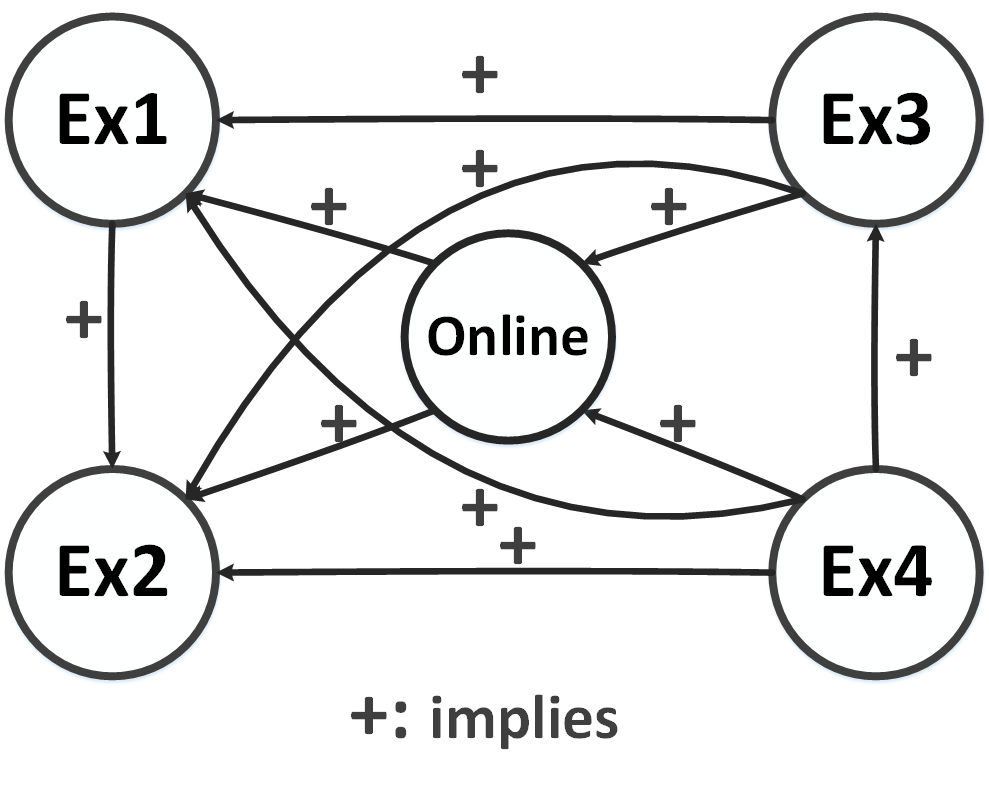
\includegraphics[scale=0.28]{figures/Fig8.png}}
	}}
      
      \caption{The implication relationships graph between existing observability 1, 2, 3, 4, and online observability where ``$\rightarrow$" means ``implies".}
      \label{fig:7}
   \end{figure}

From the implication relationships between online observability and existing observability we know that the online observability can help us solve some problem which can not be solved by existing observability. 
 \begin{itemize}
 \item Firstly, if the \BCNs\ are online observable but not satisfy the existing third and fourth observability, then the online observability can help us determine their initial state. 
 \item Secondly, it takes least observation costs for us to determine the initial state of some systems described by \BCNs. There are some biological systems depicted by \BCNs, such as the immune systems which can be depicted as the \BCN\ T-cell receptor kinetics model \cite{Klamt2006A}. And there exist input-nodes and state-nodes in this model, for the purpose of obtain the initial state of this \BCN, we must select some state-nodes to be observed at first. If we use the online observability to determine the initial state of the \BCN\ T-cell receptor kinetics model, then we need less output-nodes and then least observation costs.
 \end{itemize}

What is more, with the online observability, we can make some optimizations in the process of determining the initial state. We will represent them in the {\em Section \ref{sec:app}}.
   
   